\chapter{State of the Art}
\label{chap:stateofart}

This chapter introduces a modest introduction to the \gls{IoT} landscape. Focusing first on technologies, solutions and the architectural context surrounding them and later the various business areas where \gls{IoT} is required.
The intent of this chapter is to introduce the reader to the subjects related to this work.

\section{Internet of Things}
\label{sec:stateofart:iot}

%todo
This section has provided a short overview of IoT devices and systems. It is not designed to be comprehensive or even extensive, but simply to provide enough background to support the discussion of requirements and capabilities below.

\section{IoT Architectural Context}
\label{sec:stateofart:arch}

This section focus on the landscape of services, solutions, tools, terms and technologies that are related to \gls{IoT}.
It starts by dividing the concepts in three distinct categories:

\begin{itemize}
    \item \nameref{subsec:stateofart:arch:infra}: concepts that don't answer any specific business case but are common or even a requirement for most \gls{IoT} related projects; 
    \item \nameref{subsec:stateofart:arch:platforms}: concepts that support and ease the creation of \gls{IoT} projects but are not a necessity;
    \item \nameref{subsec:stateofart:arch:solutions}: concepts that answer specific business cases.
\end{itemize}

After these categories are explored, some \nameref{subsec:stateofart:arch:ref} are presented and correlated with some of the concepts mentioned before.

\subsection{Infrastructure} % Integration?
\label{subsec:stateofart:arch:infra}

Here some technologies and services that are almost a requirement to build \gls{IoT} Solutions are presented. This section is divided in the following themes: \nameref{subsubsec:stateofart:arch:infra:mediator}, \nameref{subsubsec:stateofart:arch:infra:middleware}, \nameref{subsubsec:stateofart:arch:infra:rule} and \nameref{subsubsec:stateofart:arch:infra:store}.

These specific themes are mentioned since they are relevant for the project.

\subsubsection{Mediator}
\label{subsubsec:stateofart:arch:infra:mediator}

This section refers to technologies that enable the system-wide use of the publish/subscribe pattern by mediating messages or events between entities of the system in a asynchronous manner.

According to \cite{DIAS2022100529}, ``broker-mediator architectures are highly used [in \gls{IoT} Solutions]'' and, the publish/subscribe ``communication pattern is also common in many IoT and Web applications'' \parencite{LAZIDIS2022100538}. 

The publish/subscribe pattern can be summarized by the following description: ``Subscribers have the ability to express their interest in an event, or a pattern of events, and are subsequently notified of any event, generated by a publisher, which matches their registered interest'' \parencite{10.1145857076.857078}.

In this section two open-source mediators, \citetitle{rabbitmq} and \citetitle{kafka}, will be introduced.

According to \cite{LAZIDIS2022100538}, RabbitMQ offers better latency than Kafka but has a significant lower throughput of messages per second.

\paragraph{RabbitMQ}
\label{par:stateofart:arch:infra:mediator:rabbitmq}

\citetitle{rabbitmq} is a message broker with support for various protocols (some via extensions) such as: (i) \gls{AMQP} 0.9.1, (ii) STOMP, (iii) \gls{MQTT}, (iv) \gls{AMQP} 1.0, (v) HTTP and WebSockets and (vi) RabbitMQ Streams. This section will focus on \gls{AMQP} 0.9.1 and \gls{MQTT}.

As discussed in the article, \citetitle{rabbitmqexpl}, the \gls{AMQP} 0.9.1 protocol defines four main concepts: (i) publisher, (ii) exchange, (iii) queue, (iv) consumer. The following diagram, Figure~\ref{fig:implementation:decisions:rabbitmq} explains how this concepts interact.

\begin{figure}[H]
    \centering
    \resizebox{\columnwidth}{!}
    {
       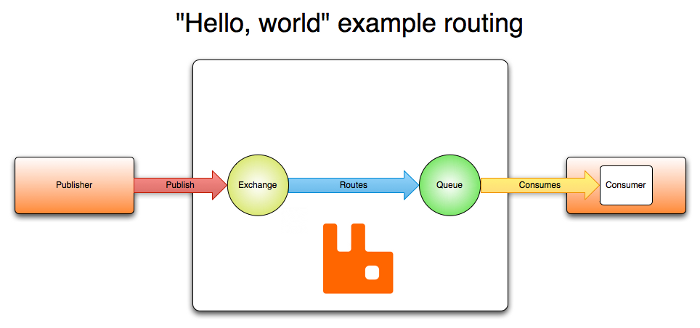
\includegraphics{assets/figures/rabbitmq.png}
    }
    \caption[\gls{AMQP} 0.9.1 Protocol Concepts]{\gls{AMQP} 0.9.1 Protocol Concepts by \cite{rabbitmqexpl}}
    \label{fig:implementation:decisions:rabbitmq}
\end{figure}

As discussed in \citetitle{rabbitmqexpl}, there are four types of exchanges:

\begin{itemize}
    \item Direct Exchange: ideal for the unicast routing of messages;
    \item Fanout Exchange: ideal for the broadcast routing of messages;
    \item Topic Exchange: ideal for the multicast routing of messages, queues subscribe to specific routing keys;
    \item Header Exchange: ideal for more flexible unicast routing of messages, queues subscribe to specific message headers.
\end{itemize}

This is the "core" protocol supported by the system.

The \gls{MQTT} protocol is a ``binary protocol emphasizing lightweight publish / subscribe messaging, targeted towards clients in constrained devices'' \parencite{rabbitmq}. According to \cite{mqtt}, this is the standard protocol for \gls{IoT} Messaging.

\cite{mqtt-vs-amqp} mentions that ``\gls{MQTT} has just one routing mechanism - topic subscriptions'', when compared with \gls{AMQP}. It can be seen as simpler version of \gls{AMQP} tailored for \gls{IoT} low powered devices. It has a lower message overhead, and instead of using \textit{'.'} as the level separator it uses a \textit{'/'}, for wildcards it uses \textit{'+'} instead of \textit{'*'}. 

Both protocols have various robust client libraries written for various programing languages \parencite{rabbitmq}. 

According to \cite{10.1145/3093742.3093908} the unique features of RabbitMQ are: (i) Standardized Protocol, (ii) Multi-protocol, (iii) Distributed Topology Modes, (iv) Comprehensive Management and Monitoring Tools, (v) Multi-tenancy and Isolation, (vi) Consumer Tracking, (vii) Disk-less Use, (viii) Publisher Flow Control, (ix) Queue Size Limits and (x) Message time to live.

\paragraph{Kafka}
\label{par:stateofart:arch:infra:mediator:kafka}

\citetitle{kafka} is a distributed event streaming platform that can be seen as an append-only-log. Its main concepts are: (i) events, (ii) producers, (iii) consumers and (iv) topics.

Events are sent by producers to specific topics that are partitioned by several Kafka brokers. Events are persisted, something that the \gls{AMQP} protocol doesn't do, and consumers can pull events from their subscribed topics. Since events are stored, a consumer can deliberately rewind back to an old offset and re-consume data \parencite{pubsubpushpull}. This enables consumers to easily follow the \citetitleyear{eventsourcing} and reconstruct an entity's current state by replaying the events.

``The Kafka ecosystem offers libraries and tools that provide additional functionality on top of Kafka'' \parencite{10.1145/3093742.3093908}, such as Kafka Connect and Kafka Streams.

According to \cite{kafkaconnect}, ``Kafka Connect works as a centralized data hub for simple data integration between databases, key-value stores, search indexes, and file systems''.

Kafka Streams ``is a client library for building applications and microservices, where the input and output data are stored in an Apache Kafka cluster. It combines the simplicity of writing and deploying standard Java and Scala applications on the client side with the benefits of Kafka's server-side cluster technology'' \parencite{kafkastreams}.

According to \cite{10.1145/3093742.3093908} the unique features of Kafka are: (i) Long term message storage, (ii) message replay, (iii) kafka connect and (iv) log compaction.

\subsubsection{IoT Middleware}
\label{subsubsec:stateofart:arch:infra:middleware}

The term \gls{IoT} Middleware in this work referes to platforms/solutions that offer or focus on three main features:

\begin{itemize}
    \item Device Management: device onboarding, maintenance, updates and monitoring;
    \item Data Transmission: device data collection and provision in real-time;
    \item Device Control: offer an \gls{API} to send commands to devices. 
\end{itemize}

These platforms handle the lower-layers communication protocols such as: (i) RFID, (ii) Bluetooth/BLE, (iii) LoRa and LoRaWAN, (iv) SigFox, (v) ZigBee, (vi) Thread, (vii) EnOcean, (viii) ANT, (ix) GPRS/2G/3G/4G/5G cellular, (x) Wi-Fi \parencite{DIAS2022100529}.

The article \citetitleyear{DIAS2022100529} argues that due to a lack of standards a designer can't objectively choose from one or another protocol when developing \gls{IoT} Systems. These platforms have the benefit of abstracting these lower-layers communication details and provide \gls{API}s that provision all data gathered with high-layer communication protocols like (i) HTTP, (ii) \gls{MQTT}, (iii) \gls{AMQP}, (iv) CoAP, (v) XMPP, (vi) LwM2M, (vii) LLAP, (viii) UPnP \parencite{DIAS2022100529}.

The platforms that will be briefly mentioned are:

\begin{itemize}
    \item \nameref{par:stateofart:arch:infra:middleware:ttn};
    \item \nameref{par:stateofart:arch:infra:middleware:azure};
    \item \nameref{par:stateofart:arch:infra:middleware:helium}.
\end{itemize}

This project focus mostly on \nameref{par:stateofart:arch:infra:middleware:helium} since it controls the lower-layers communication with the company's installed devices (via the community's installed hotspots).

\paragraph{The Things Stack}
\label{par:stateofart:arch:infra:middleware:ttn}

\citetitleyear{ttn} is behind the creation of a platform that focus on interacting with devices via LoRa and LoRaWAN.

Apart from the common features referred above, their cloud platform provides integrations with AWS IoT, Azure IoT Hub and other platforms such as Cumulocity, ThingsBoard, and LoRa Cloud. It also provides agnostic \gls{API}s based on \gls{MQTT}, webhooks and PubSubs to connect with other systems and publish the gathered device measures.

The company maintains an open-source version of their platform. According to \citetitleyear{ttn-stack}, this platform supports: almost all the LoRaWAN protocols specifications, device classes, regional parameters and onboarding options; device payload conversion for well-known formats or via custom Javascript functions; user and entity management; and GRPC and HTTP management \gls{API}s. 

\paragraph{Azure IoT Hub}
\label{par:stateofart:arch:infra:middleware:azure}

\citetitleyear{azure-hub} is a platform provided by Microsoft ``that acts as a central message hub for communication between an IoT application and its attached devices'' \parencite{azure-hub}. A helper service, Azure IoT Hub Device Provisioning Service, handles the registration and provisioning of devices.

According to \cite{azure-hub} data can also be routed to different services for further processing, it is possible to route data to: azure storage containers, event hubs, service bus queues and services bus topics. According to \cite{azure-hub-amqp}, it is also possible to subscribe to an \gls{AMQP} endpoint to receive the device measures sent to \gls{IoT} Hub. Azure IoT Hub also integrates with Azure Event Grid that allows one to register an HTTP endpoint for Azure Event Grid to dispatch events to, in this case, device measures.

According to \citetitleyear{azure-gartner}, Azure is a leading \gls{IoT} Platform.

\paragraph{Helium Console}
\label{par:stateofart:arch:infra:middleware:helium}

\citetitleyear{helium} is a new \gls{IoT} Platform. This platform's business model is fairly different from the ones mentioned before. Besides the platform itself, the company also maintains an open-source blockchain designed to power \gls{IoT} devices with wireless connectivity. Helium technology enables communication between devices and the internet by promoting the expansion of a new network operated by common people.

According to \cite{helium-wp}, `` Powering the Helium network is a blockchain with a native protocol token incentivizing a two-sided marketplace between coverage providers and coverage consumers''. Coverage providers install in their homes an \gls{IoT} gateway, Hotspot, that provides wide-area LoRaWAN coverage to the area surrounding it. Coverage consumers, e.g. \gls{IoT} devices, connect to this LoRaWAN network and send the gathered measures to the Hotspot. The Hotspot them routes the measures to the cloud in exchange for a transport fee, paid by the owner of the \gls{IoT} device.
The fee corresponds to a token that can be traded for dollars, bitcoin or any other available commodity on online exchanges.

In theory, this creates a self sustained economy that can provide to everyone a cheap and open communication layer for \gls{IoT} devices that is backed by open standards, and, provide a consistent income to those who what to support the network. The \textit{Helium Explorer Page}\footnote{\href {https://explorer.helium.com/}{link to Helium Explorer Page}} documents the number and location of each Hotspot, current there are almost a million of \gls{IoT} gateways installed throughout the world. Europe, USA and China are the regions with better network coverage.

This network, as an example, gives local farmers in remote locations the possibility to install a smart irrigation system without paying excruciating fees to an \gls{ISP} for satellite or 4G coverage.

The company's business idea is to utilize this low-cost network to offer \gls{IoT}-based services to small-to-medium size organizations.
Therefore, the solution to develop in this project will, at least in the near future, focus on the \gls{IoT} Middleware solution provided by Helium.

Helium Console enables devices to connect to pre-configured, cloud-based applications or send data directly over HTTP or MQTT via Integrations.
It currently supports two core integrations, HTTP and \gls{MQTT}, and multiple community integrations such as: (i) Helium Cargo, (ii) myDevices Cayenne, (iii) AWS IoT Core, (iv) Azure IoT Hub, (v) Azure IoT Central, (vi) Adafruit IO, (vii) Akenza, (viii) Datacake, (ix) Google Sheets, (x) Microshare, (xi) TagoIO, (xii) Ubidots \parencite{helium-integrations}. 

\subsubsection{Data Storage}
\label{subsubsec:stateofart:arch:infra:store}

This section refers to how information is stored and managed across systems.

A \gls{DBMS} is a general-purpose software system that facilitates the processes of defining, constructing, manipulating, and sharing data - \citetitle{elmasri2000fundamentals}. \gls{DBMS}s can be categorized according to several criteria, such as the data model, number of users or distribution. This section focus on the data model.

These are some of the data model types, according to \cite{elmasri2000fundamentals}:

\begin{itemize}
    \item The \textbf{relational data model} represents a database as a collection of tables, where each table can be stored as a separate file;
    \item The \textbf{document-based data model} is based on JSON (Java Script Object Notation) and stores the data as documents, which somewhat resemble complex objects;
    \item The \textbf{column-based data model} stores the columns of rows clustered on disk pages for fast access and allow multiple versions of the data;
    \item The \textbf{graph-based data model} stores objects as graph nodes and relationships among objects as directed graph edges;
    \item The \textbf{key-value data model} associates a unique key with each value (which can be a record or object) and provides very fast access to a value given its key.
\end{itemize}

The following sections briefly discuss these data models.

\paragraph{Relational Data Model}
\label{par:stateofart:arch:infra:store:relational}
%todo: main info
This data model has a wide variety of usage in the industry. Some of the technologies that follow this data model are: (i) \citetitle{mysql}, (ii) \citetitle{postgressql} and (iii) \citetitle{mariadb}.

It is intended for strictly structured data with well defined interrelations.

\subsubsection{Document-based Data Model}
\label{par:stateofart:arch:infra:store:nosql}
%todo: main info
This data model rose from the increasing need to store and analyze unstructured data as stated by \cite{miloslavskaya2016big}.  Citing \cite{elmasri2000fundamentals}, a ``major difference between document-based systems versus object and object-relational systems (relational database systems) is that there is no requirement to specify a schema''.

\subsubsection{Column-based Data Model}
\label{par:stateofart:arch:infra:store:time}

This data model is used in applications that require large amounts of data storage, and is commonly named \textit{data warehouses}. According to \cite{dehdouh2015using}, a data warehouse  is ``designed according to a dimensional modelling which has for objective to observe facts through measures, also called indicators, according to the dimensions that represent the analysis axes''. Citing \cite{han2011survey}, these databases ``can maintain high-performance of data analysis and business intelligence processing''.

Some of the technologies related to this concept are: (i) \citetitle{hbase}, (ii) \citetitle{cassandradb}, (iii) \citetitle{influxdb}, (iv) \citetitle{questdb}.

According to \cite{george2011hbase} HBase is a ``distributed, persistent, strictly consistent storage system with near-optimal write and excellent read performance''. This database uses \gls{HDFS} as its file system, and so, it is built on top of Hadoop.
HBase does not support a structured query language like \gls{SQL}, ``even though it's comprised of a set of standard tables with rows and columns, much like a traditional database'' (\cite{ibm-hbase}).

CassandraDB is a distributed storage system for managing very large amounts of structured data spread out across many commodity servers, while providing highly available service with no single point of failure (\cite{lakshman2010cassandra}).
It was developed internally by Facebook and then later open-sourced to the Apache Foundation. It doesn't support \gls{SQL}.

According to \cite{naqvi2017time}, InfluxDB is an ``open-source schemaless \gls{TSDB} with optional closed-sourced components developed by InfluxData. It is written in Go programming language and it is optimized to handle time series data.'' It provides an SQL-like query language and also defines a new protocol for fast data ingestion (\cite{ilp}).

QuestDB is a relational column-oriented database designed for time series and event data and entitles it self as the ``fastest open source time series database'' (\cite{questdb}).
According to benchmarks (\cite{quest-bench}) preformed using the \gls{TSBS}, \cite{TSBS}, QuestDB ranks as the fastest option in the market.
It has out-of-the-box support for SQL Postgres wire protocol, (thus integrating with \citetitle{postgressql} client libraries), can be easily deployed using a single Docker Image, and also supports the \gls{ILP}.

\subsubsection{Graph-based Data Model}
\label{par:stateofart:arch:infra:store:graph}

\subsubsection{Key-Value Data Model}
\label{par:stateofart:arch:infra:store:key}

\subsubsection{Rule Engine}
\label{subsubsec:stateofart:arch:infra:rule}

\subsection{Platforms}
\label{subsec:stateofart:arch:platforms}

Things Board

TagoIO

DataCake

Node-red

\subsection{Solutions}
\label{subsec:stateofart:arch:solutions}

This section focus on several solutions devoted to specific business cases.
The objective of this section is to simply introduce the major features of the solutions, how they work and what is the business model behind their company, when applicable.

The business cases addressed here are the ones this project attempts to answer.

\subsubsection{Indoor Fire Detention}
\label{subsubsec:stateofart:arch:solutions:fire}

\subsubsection{Smart Irrigation}
\label{subsubsec:stateofart:arch:solutions:irrigation}

This section mentions some Smart Irrigation Solutions discussed by \cite{OBAIDEEN2022100124}.

According to \cite{8372905} a Smart Irrigation System offers the following benefits: (i) Community Farming, (ii) Safety Control and Fraud Prevention, (iii) Competitive Advantages, (iv) Wealth Creation and Distributions, (v) Cost Reduction and Wastage, (vi) Operational Efficiency, (vii) Awareness and (ix) Asset Management.

As for the solutions:

WaterBit provides a ``secured wireless connectivity to its autonomous irrigation solution, allowing management and control of local irrigation'' \parencite{OBAIDEEN2022100124}. WaterBit gathers soil moisture levels measured every few minutes and presents theses measures via a mobile-friendly application where farmers can control the irrigation system.

Ipswich city council ``depicted that using an automated soil-moisture monitoring system as a driver of irrigation leads to significantly conserve water along with saving costs'' \parencite{OBAIDEEN2022100124}. The system's method to control the irrigation system was considered highly efficient when compared with a rainfall-based allocation method.

Maejo University in Thailand built a system to control the environment where mushrooms were cultivated. The system measured light, air temperature, air humidity and air flow to determine when to activate the irrigation system \parencite{OBAIDEEN2022100124}. The system was powered by solar energy.

AgirSens is a dynamic irrigation scheduling system based on IoT for efficient water management of irrigated crop fields. According to \cite{9249427} ``AgriSens has a farmer-friendly user interface, which provides field information to the farmers in a multimodal manner - visual display, cell phone, and Web portal''.

\subsubsection{Fleet Management}
\label{subsubsec:stateofart:arch:solutions:fleet}

This section focus on some Fleet Management and Asset Tracking solutions. No relevant papers were found regarding the use of \gls{IoT} in Fleet Management or Asset Tracking solutions, therefore the solutions here presented were gathered by the author based on the quality of information available regarding their company's business model, iot devices used and features offered.

As for the solutions:

Verizon Connect is a Fleet Management solution that provides it's own sensors/devices, platform and application under a subscription \parencite{verizon-iot}.
A team from Verizon installs the devices in the fleet according to the specification and access to the platform is given. This is an Hassle-free solution but the costs associated with it can be high. Since Verizon is a telecommunications conglomerate the protocols used to transport measures from devices to their platform is GPRS/2G/3G/4G/5G cellular.

SmartDrive is a Fleet Management solution that also provides it's own hardware, SR4, platform and application under a subscription. The SR4 is composed by a controller (solid-state storage, multiple communication protocols, advanced driver assistance system functions, computer-vision aided processing requirements), cameras, sensor bar (GPS, accelerometers, microphone and driver-support LEDs), keypad (for manual event recording and privacy mode initiation) and Wireless Key Fob (initiate a manual recording event, both inside and outside the vehicle) \parencite{smartdrive-iot}. With all the data gathered, their platform, Transportation Intelligence Platform, is capable of ``delivering breakthrough driving performance insights and analytic intelligence'', and ``helping fleets improve fleet safety and efficiency, and manage an entirely new set of business challenges arising in the future'' \parencite{smartdrive-iot2}.

LocaTrack is a platform for Asset Tracking built by Safecube \parencite{safecube}, this service provides the following Key Features: 

\begin{itemize}
    \item Geolocation: Distance, traveled road and availability;
    \item Asset use rate analysis: better visibility on the use of assets;
    \item Optimization: detailed analysis to optimize the use of assets;
    \item Real-time alert: real-time alerts on movements, geofencing, sleeping assets and others;
    \item Prediction: Maintenance, Servicing and Asset location;
    \item Condition monitoring: IoT trackers can detect changes in temperature, humidity or shocks and others.
\end{itemize}

According to \cite{safecube-azure}, LocaTrack uses SigFox for lower-level communication and Azure IoT Hub to collect the location of tracked assets.

Finally, TrackPac is a service for asset tracking \parencite{trackpac}. This service offers an application that presents real-time location data, battery data and geofence alerts of the managed assets. By using LoRaWAN (provided by Helium, the same network used in this project) for lower-level communication it promises a service ten times cheaper than the ones that require 4G. This service works with LoRaWAN class A trackers and does not enforce the use of any proprietary, close-source devices even though it recommends the use of Browan Tabs Object Locator, Digital Matter Oyster3 or Abeeway Micro. 

\subsection{Reference Architectures}
\label{subsec:stateofart:arch:ref}

As the \gls{IoT} domain covers such a wide spectrum of application fields with very little in common, the development cycles, technologies and architectures used can be completely different. The vast array of choices given to those involved in a greenfield project of this area, coupled with the lack of standards with a broad usage \parencite{DIAS2022100529, weyrich2015reference}, can linger the design, development and interoperability of \gls{IoT} systems.

Reference Architectures for the \gls{IoT} aim to help developers tackle some of these problems \parencite{weyrich2015reference}.

According to \cite{muller2008reference}, a Reference Architecture ``captures the essence of the architecture of a collection of systems. The purpose of a Reference Architecture is to provide guidance for the development of architectures for new versions of the system or extended systems and product families''.

This section sheds a light on some of the Reference Architectures of this field, what their focus is and the relevancy they have for this project.

The Reference Architectures discussed are: (i) \nameref{subsubsec:stateofart:arch:iota}, (ii) \nameref{subsubsec:stateofart:arch:sat}, (iii) \nameref{subsubsec:stateofart:arch:iira}, (iv) \nameref{subsubsec:stateofart:arch:wso2}, (v) \nameref{subsubsec:stateofart:arch:p2413}, (vi) \nameref{subsubsec:stateofart:arch:rami}, (vii) \nameref{subsubsec:stateofart:arch:azure}, (viii) \nameref{subsubsec:stateofart:arch:arrrowhead}.

This section was based on the papers written by \cite{Lynn2020} and \cite{DIAS2022100529}.

Intel System Architecture Specifications (Intel SAS) will not be discussed since no relevant information was found about it.
The \nameref{subsubsec:stateofart:arch:iota} also mentions the \gls{IoT} \gls{ARM}.

\subsubsection{IoT-A}
\label{subsubsec:stateofart:arch:iota}

The IoT Architecture goals are to create ``an architectural reference model for the interoperability of Internet-of-Things systems, outlining principles and guidelines for the technical design of its protocols, interfaces, and algorithms'' that shall ``lead to corresponding mechanism for its efficient integration into the service layer of the Future Internet''. \parencite{iot-a}. This project's final version is dated back to July 2013.

It defines a collection of Unified Requirements that support and validate concrete architectures created according to the \gls{IoT} \gls{ARM}. Some of these requirements were also applied to this project.

According to \cite{krvco2014designing}, this project motto is ``to offer IoT architects a common technical grounding in order to optimize interoperability. In that case, IoT applications would not be any longer built as stand-alone silo applications, but as inter-operable vertical applications still having a common "horizontal" grounding - the \gls{ARM} (compliant components, protocol suites, etc.)''.

This project originated the \gls{IoT} \gls{ARM} that can be divided into three interconnected parts \parencite{krvco2014designing}:

\begin{itemize}
    \item The IoT Reference Model;
    \item The IoT Reference Architecture;
    \item A set of Guidance (also called best practice).
\end{itemize}

The reference model defines several models that help to describe certain aspects of the \gls{IoT} architecture, some of this models are described by \cite{6682101}. It defines five core concepts:

\begin{itemize}
    \item Augmented Entity: a combination of a Physical Entity (real world object) and its Virtual Entity (digital representation);
    \item User: Those who interact with the system, human beings, devices, services and others;
    \item Device: Hardware to monitor or interact with real world objects;
    \item Resource: Computational element that gives access to information or control over a real-world object;
    \item Service: Entities that expose resources via a common interface, making then available for consumption by other services.
\end{itemize}

Each concept is them explored in detail. These concepts are them used to create the reference architecture.

According to \citetitleyear{iot-arm}, ``the Reference Architecture can be visualized as the "Matrix" that eventually gives birth ideally to all concrete architectures''. ``Guidance in form of best practices can be associated to a reference architecture in order to derive use-case-specific architectures from the reference architecture''.

The IoT Reference Architecture provides a functional view, presented in the Figure~\ref{fig:stateofart:arch:iota:functional}.

\begin{figure}[H]
    \centering
    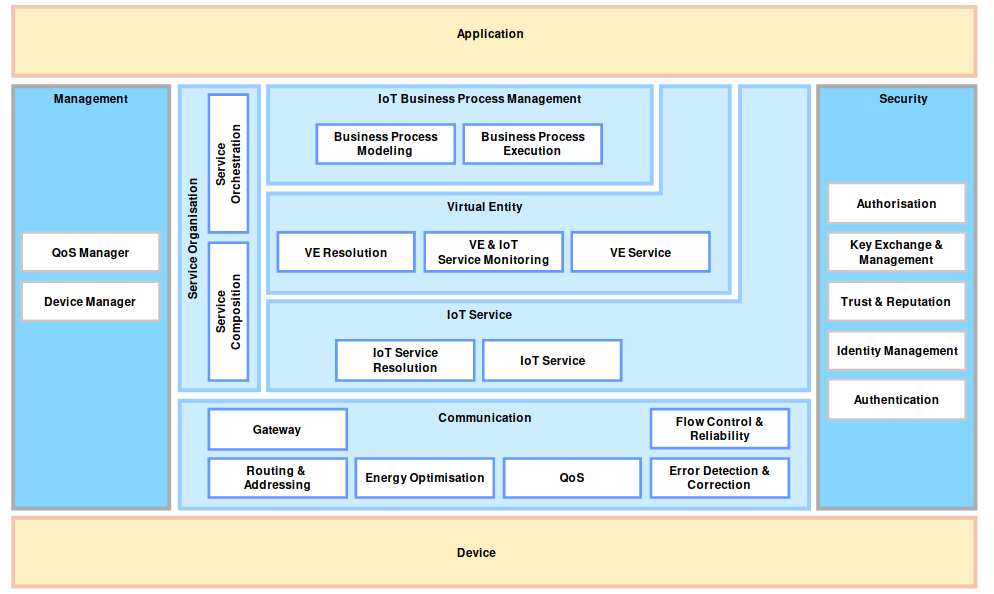
\includegraphics[scale=0.5]{
        assets/figures/arm-functional-view.png
    }
    \caption[ARM Functional View]{ARM Functional View, \cite{iot-arm-functional}}
    \label{fig:stateofart:arch:iota:functional}
\end{figure}

This functional view divides the architecture of a system in various functional components with well defined concerns.

\subsubsection{SAT-IoT}
\label{subsubsec:stateofart:arch:sat}

\cite{8767282} present an architectural model definition that lead to the development of ``a new advanced \gls{IoT} platform referred as SAT-IoT''. This model attempts to integrate concepts such as:  ``the paradigm of edge/cloud computing transparency, the IoT computing topology management, and the automation and integration of IoT visualization systems''. This project's final version is dated back to 2019, it apeares that the envisioned platform was not implemented since no other reference to it was found.

The diagram in Figure~\ref{fig:stateofart:arch:sat:model} defines the concepts, services and relations of this model.

\begin{figure}[H]
    \centering
    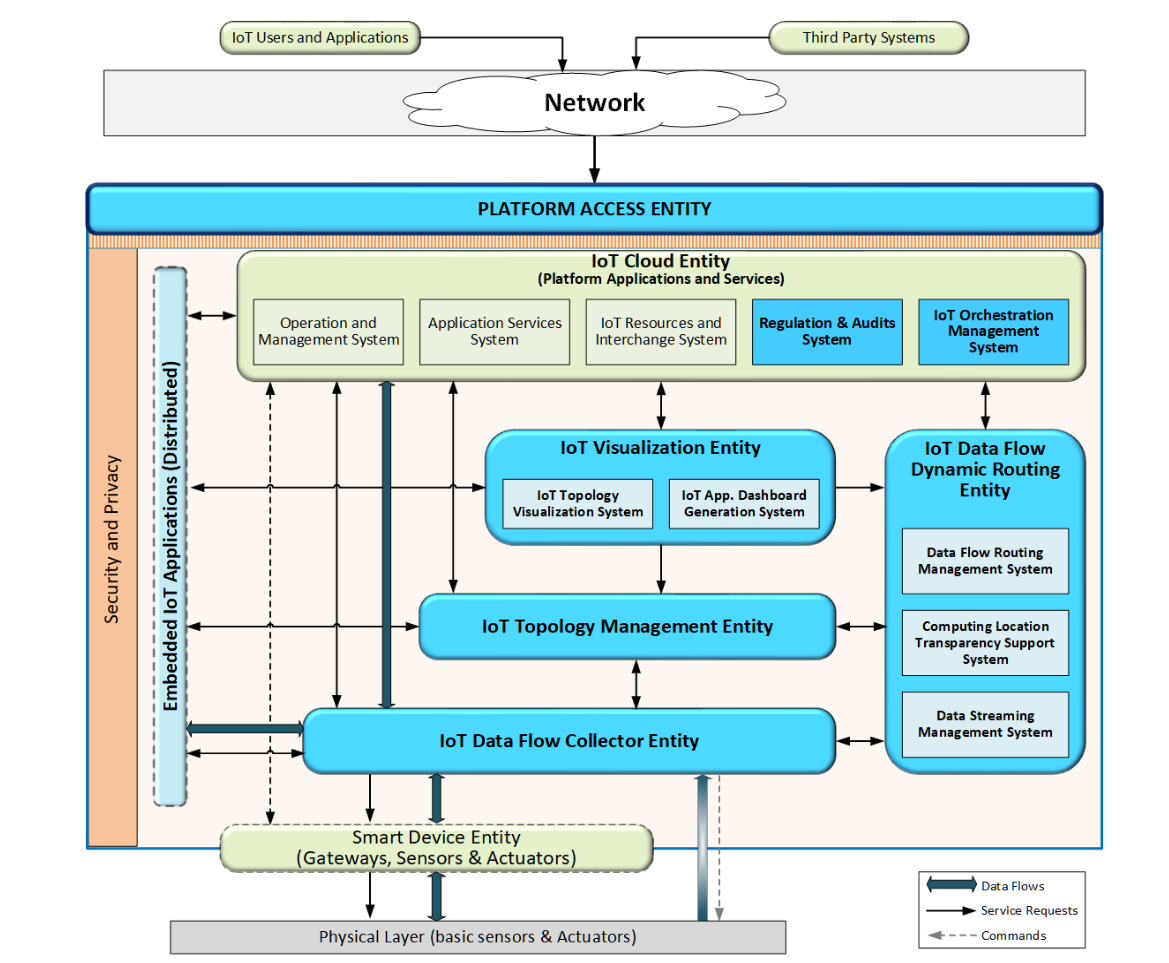
\includegraphics[scale=0.4]{
        assets/figures/sat-iot.png
    }
    \caption[SAT-IoT Architectural Model]{SAT-IoT Architectural Model, \cite{8767282}}
    \label{fig:stateofart:arch:sat:model}
\end{figure}

This model focus on a distributed system with a tree-like structure, where data can be dynamically processed in different node levels (edge, mid or cloud) in order to optimize response latency, bandwidth consumption, storage and other metrics. Components such as "IoT Topology Management Entity", "IoT Data Flow Dynamic Routing Entity" and "IoT Visualization Entity" focus on optimally distributing the workload across all nodes of the system.

The architecture also enables one to host "Embedded IoT Applications" that have full access to the system internals, leading to strongly integrated applications.

\subsubsection{IIRA}
\label{subsubsec:stateofart:arch:iira}

The \gls{IIRA} ``addresses the need for a common architecture framework to develop interoperable IIoT systems for diverse applications across a broad spectrum of industrial verticals in the public and private sectors to achieve the true promise of IIoT'' \parencite{iira}. This project's final version is dated back to June 2019.

It decomposes a typical Industrial \gls{IoT} system in five distinct functional domains:

\begin{itemize}
    \item \textbf{Control Domain}: this domain focus on functions that are performed by industrial control and automation systems. It is deployed in proximity to the physical systems and therefore geographically distributed;
    \item \textbf{Operations Domain}: this domain focus on the management and operation of the control domain. It should be able to configure, register, track and control assets. It is also responsible for providing real-time prognostics, monitoring and diagnostics of the managed assets;
    \item \textbf{Information Domain}: this domain is responsible for managing and processing data, it should transform, persist, and model or analyze data to acquire high-level intelligence about the overall system;
    \item \textbf{Application Domain}: this domain is responsible for applying business focused rules and logic to the gathered information;
    \item \textbf{Business Domain}: this domain is responsible for implementing business processes, such as Enterprise Resource Planning, Costumer Relationship Management, Manufacturing Execution System, Billing and Payment, Work Planning and Scheduling Systems. 
\end{itemize}

These domains interact according to Figure~\ref{fig:stateofart:arch:iira:domains}.

\begin{figure}[H]
    \centering
    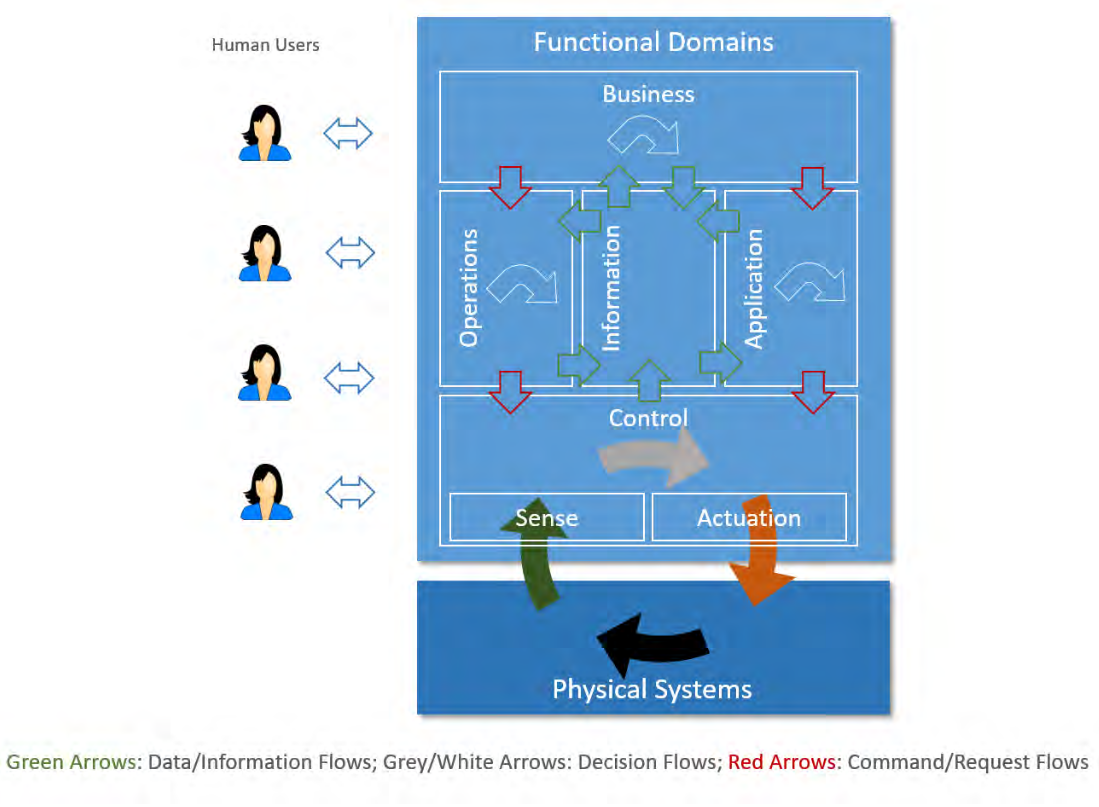
\includegraphics[scale=0.5]{
        assets/figures/irra-domains.png
    }
    \caption[\gls{IIRA} Functional Domains]{\gls{IIRA} Functional Domains, \cite{iira}}
    \label{fig:stateofart:arch:iira:domains}
\end{figure}

As information flows from the control domain to the business domain it is enriched, cleaned, filtered and combined leading to a broader and richer notion of the complete environment. New information can be derived, and new intelligence may emerge from this broader information.

When applied to the common three tier architecture for IoT systems, these domains are organized according to Figure~\ref{fig:stateofart:arch:iira:applied}.

\begin{figure}[H]
    \centering
    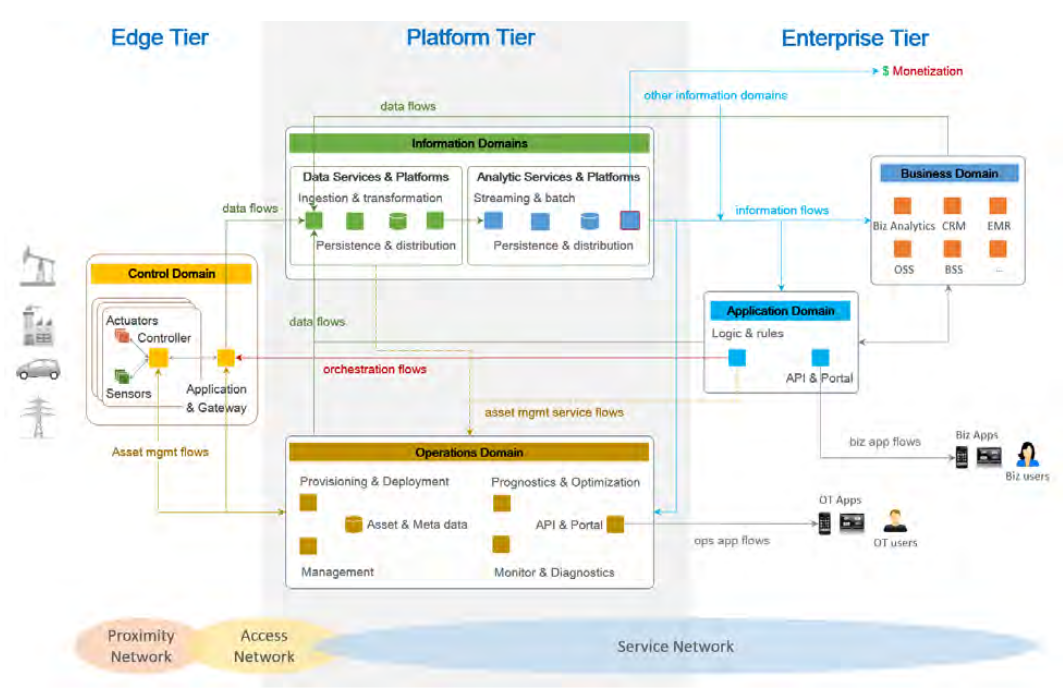
\includegraphics[scale=0.5]{
        assets/figures/irra-applied.png
    }
    \caption[Mapping between a three tier architecture and the \gls{IIRA} function domains]{Mapping between a three tier architecture and the \gls{IIRA} function domains, \cite{iira}}
    \label{fig:stateofart:arch:iira:applied}
\end{figure}

\subsubsection{WSO2 IRA}
\label{subsubsec:stateofart:arch:wso2}

The WSO2 reference architecture aims to ``provide an architecture that supports integration between systems and devices'' \parencite{wso2ira}. This project's final version is dated back to October 2015.

It groups the \gls{IoT} related requirements in the following key categories: (i) Connectivity and communications, (ii) Device management, (iii) Data collection, analysis, and actuation, (iv) Scalability, (v) Security, (vi) high-availability, (vii) Predictive analysis and (viii) Integration.

This categories gave birth to the following reference architecture, Figure~\ref{fig:stateofart:arch:wso2:ra}.

\begin{figure}[H]
    \centering
    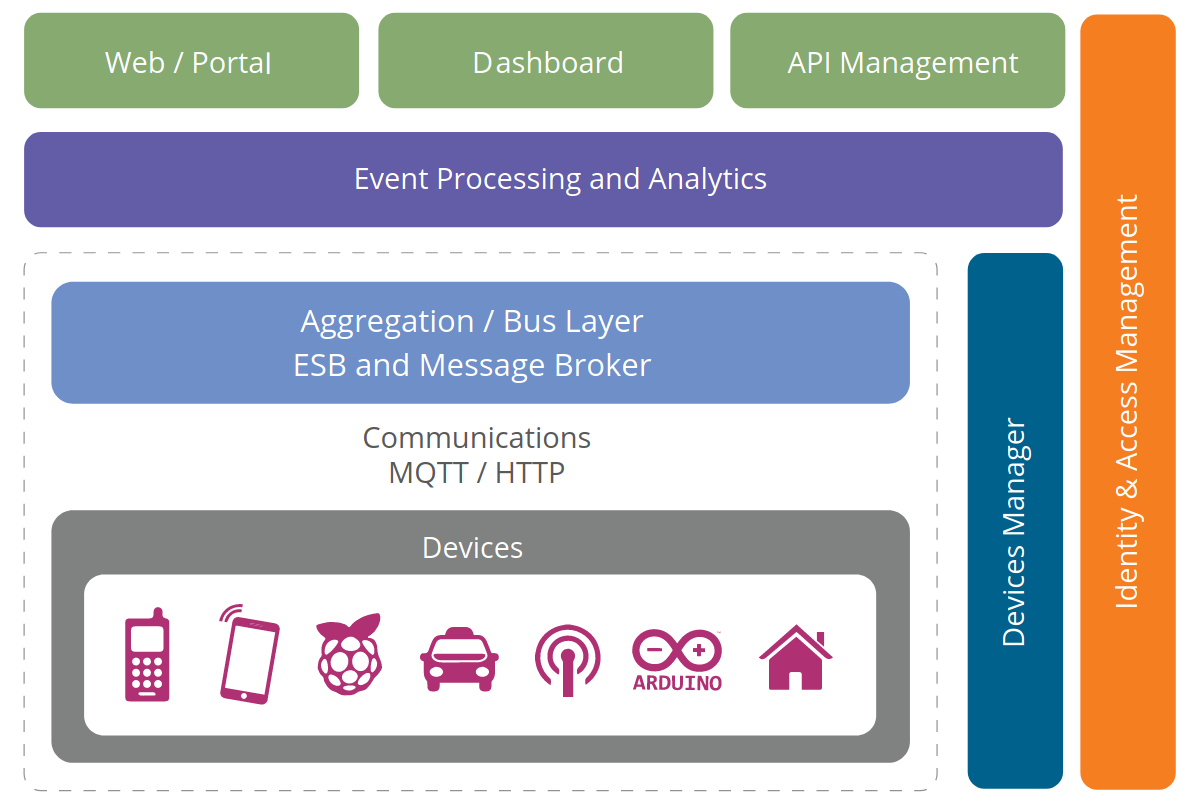
\includegraphics[scale=0.4]{
        assets/figures/wso2-ira.png
    }
    \caption[WSO2 Reference Architecture for IoT]{Reference Architecture for IoT, \cite{wso2ira}}
    \label{fig:stateofart:arch:wso2:ra}
\end{figure}

This reference architecture envisions two cross-cutting and five horizontal layers:

\begin{itemize}
    \item \textbf{Device Layer} (in grey): related to the physical \gls{IoT} devices;
    \item \textbf{Communications Layer} (without any representative color): related to the connectivity of devices;
    \item \textbf{Aggregation/bus Layer} (in light blue): related to the aggregation and supply of data upstream, bridging between the protocols used in upstream layers and downstream layers; 
    \item \textbf{Event processing and Analytics Layer} (in purple): related to data processing, analysis and storage;
    \item \textbf{Client/external Communications Layer} (in green): related to web-based frontends and portals that interact with the Event processing and Analytics layer, dashboards that
    offer views into analytics and event processing, and \gls{API}s for machine to machine communication;
    \item \textbf{Device Management Layer} (in dark blue): related to the management, onboarding and remote control of devices;
    \item \textbf{Identity Access Management} (in orange): related to the authentication and authorization of users and systems that interact with the system.
\end{itemize}

In the Event processing and analytics Layer it's recommended the use of ``a highly scalable, column-based data storage for storing events'', ``map-reduce for long-running batch-oriented processing of data'', ``complex event processing for fast in-memory processing and real-time reaction and autonomic actions based on the data an activity of devices and other systems'' and ``traditional application processing platforms'' (custom-made applications for data processing).

\subsubsection{IEEE P2413}
\label{subsubsec:stateofart:arch:p2413}

The IEEE Standard for an Architectural Framework for the IoT ``defines an architecture framework description for \gls{IoT}''. The architecture framework defined in the standard ``will promote cross-domain interaction, aid system
interoperability and functional compatibility, and further fuel the growth of the IoT market'' \parencite{9032420}.  This project's final version is dated back to June 2020.

Its architecture framework covers the definition of basic architectural building blocks and their ability to be integrated into multi-tiered systems. It describes different detailed viewpoints of the framework \parencite{9032420}:

\begin{itemize}
    \item \textbf{Conceptual Viewpoint}: concerned with defining a common vocabulary and semantics regarding a \gls{IoT} System to ease the communication across teams and encourage the reuse of concepts;
    \item \textbf{Compatibility Viewpoint}: concerned with the compatibility between systems and devices to lower the cost of integration. This viewpoint urges for the creation of new standards and compliance with those standards. It defines six levels of compatibility focused specially on physical devices: (i) incompatible, (ii) coexistent, (iii) inter connectable, (iv) inter workable, (v) interoperable and (vi) exchangeable;
    \item \textbf{Lifecycle Viewpoint}: concerned with a system's assurance, performance, maintainability and evolvability across its lifecycle: design, development, production, support, upgrade and retirement; 
    \item \textbf{Communication Viewpoint}: concerned with how devices can exchange information with each other and \gls{IoT} systems in a accurate, precise and effective manner;
    \item \textbf{Information Viewpoint}: concerned with how information is semantically defined, structured, stored, shared, manipulated, managed, and distributed across the IoT system. This viewpoint should focus on documenting system-level information, e.g., information exchanged between the various subsystems;
    \item \textbf{Function Viewpoint}: concerned with how devices can function according to their intended purpose or characteristic action, such as actuation, sensing, analysis, or control of entities of interest; 
    \item \textbf{Thread model Viewpoint}: concerned with identifying potential threats that could exploit vulnerabilities in the device, network or subsystems that encapsulate the \gls{IoT} system;
    \item \textbf{Security and safety monitoring Viewpoint}: concerned with monitoring the events occurring in an \gls{IoT} system and analyzing them for signs of possible incidents, which are violations or imminent threats of violation of security, safety, or acceptable use policies, or standard security practices;
    \item \textbf{Access control Viewpoint}: concerned with permitted activities of legitimate users, mediating every attempt by a user to access a resource in the IoT system. It is composed by three security functions: identification, authentication and authorization;
    \item \textbf{Privacy and trust Viewpoint}: concerned with the privacy of individuals or groups and trust in systems or organizations. In a complex \gls{IoT} system, arbitrary device data can be grouped and analyzed to determine the users activities;
    \item \textbf{Collaboration Viewpoint}: concerned with the collaboration of systems that belong to different application domains;
    \item \textbf{Computing resource Viewpoint}: concerned with the computing resources needed to support the \gls{IoT} system as a whole, such as gateways, data centers, \gls{PLC}s and \gls{DCS} controllers, microcontrollers embedded in sensors and actuators or others.
\end{itemize}

The idealized \gls{IoT} System should be examined according to these viewpoints in order to better define its architecture.

\cite{9032420} then procedes to define the Standard for a Reference Architecture for Smart Cities in P2413.1, the major focus of this project's business cases.

One of the architectures proposed in the standard and derived from the architecture framework is presented in Figure~\ref{fig:stateofart:arch:p2413:rasc}. 

\begin{figure}[H]
    \centering
    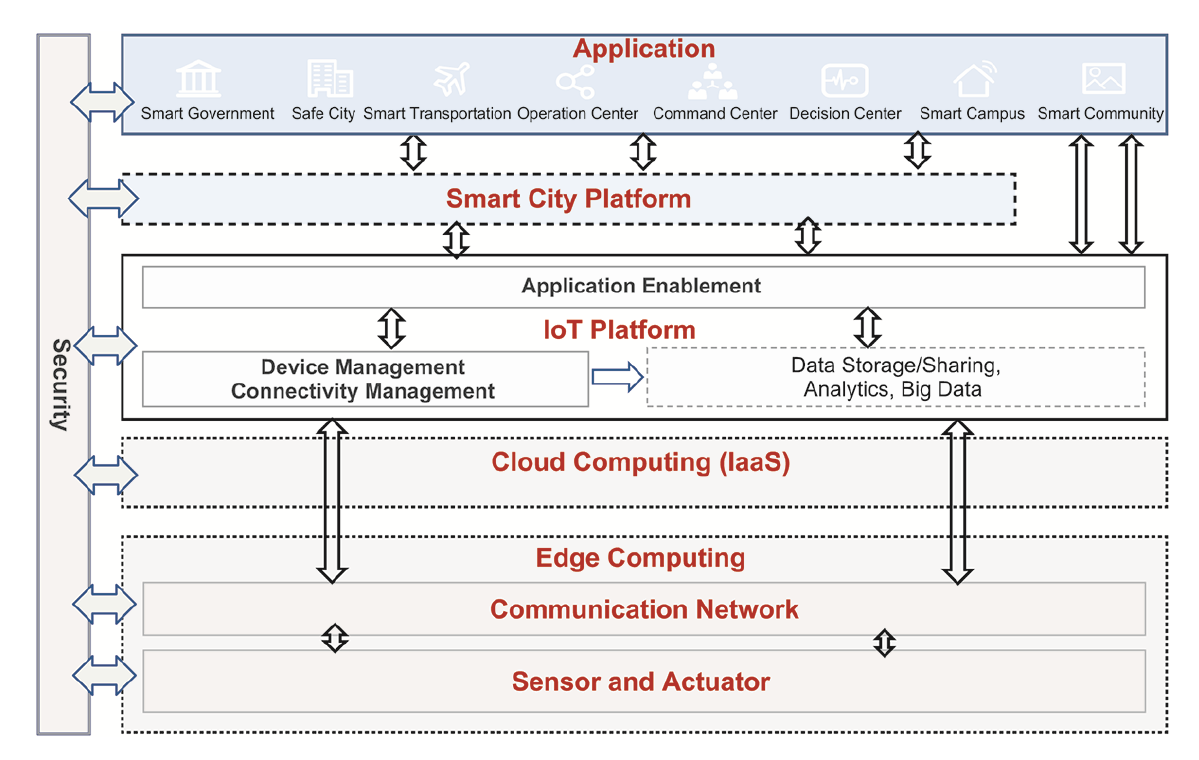
\includegraphics[scale=0.4]{
        assets/figures/smart-city-p2413.png
    }
    \caption[Example of an \gls{IoT} System Architecture for Smart Cities]{Example of an \gls{IoT} System Architecture for Smart Cities, \cite{9032420}}
    \label{fig:stateofart:arch:p2413:rasc}
\end{figure}

This architecture, derived from the common three tier architecture for \gls{IoT} Systems, proposes a new tier entitled Smart City Platform, in it ``Northbound APIs support diverse vertical applications development and southbound APIs connect to different IoT Platforms'' \parencite{9032420}.

\subsubsection{RAMI 4.0}
\label{subsubsec:stateofart:arch:rami}

The Reference Architectural Model Industry 4.0 ``ensures that all participants involved share a common perspective and develop a common understanding'' and is represented by a ``three-dimensional map showing the most important aspects of Industrie 4.0'' \parencite{hankel2015reference}. It represents a service-oriented architecture according to the manufactures association that defined it. This project's final version is dated back to August 2018 and has clear focus on the \gls{IoT} business area related to the Industry, e.g. smart factories.

The three-dimensional map is depicted in Figure~\ref{fig:stateofart:arch:rami:map}.

\begin{figure}[H]
    \centering
    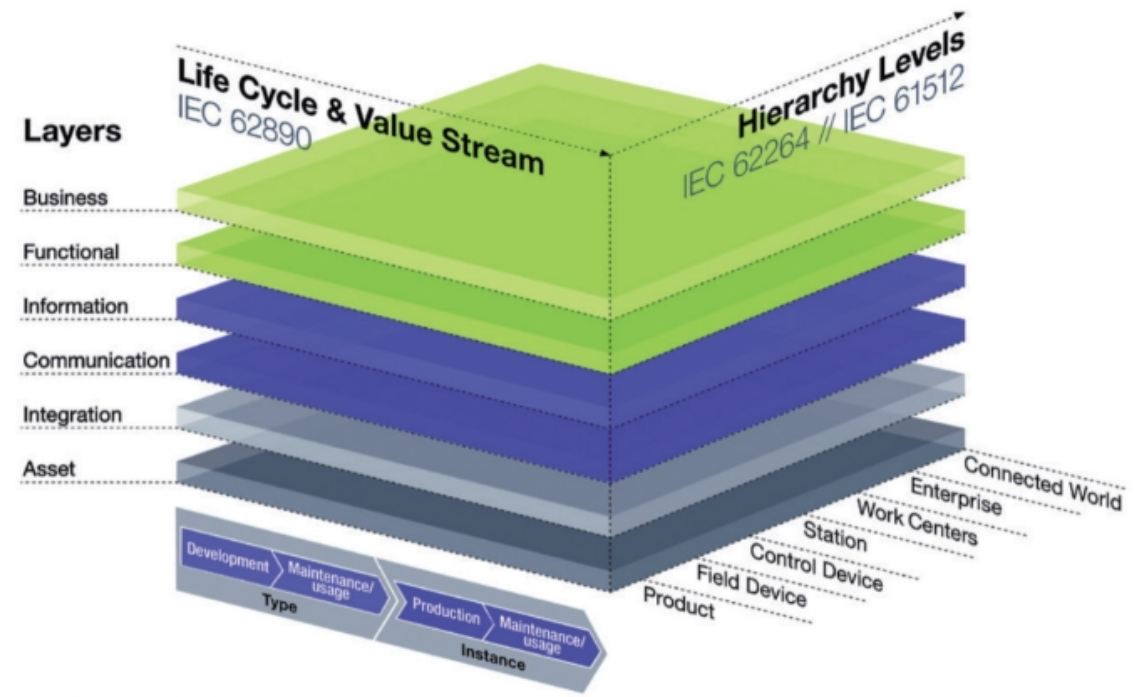
\includegraphics[scale=0.4]{
        assets/figures/rami.png
    }
    \caption[RAMI 4.0 Three-dimensional map]{RAMI 4.0 Three-dimensional map, \cite{rami}}
    \label{fig:stateofart:arch:rami:map}
\end{figure}

According to \cite{rami-explained} it is comprised of six architecture layers stretched across the hierarchy and life cycle axes:

\begin{itemize}
    \item \textbf{Business Layer}: concerned with Organization and Business processes;
    \item \textbf{Functional Layer}: concerned with the Functions of assets;
    \item \textbf{Information Layer}: concerned with the processing of the necessary data; 
    \item \textbf{Communication Layer}: concerned with how to gain access to the information needed;
    \item \textbf{Integration Layer}: concerned with the transition from things to the digital world;
    \item \textbf{Asset Layer}: concerned with the physical things in the real world.
\end{itemize}

This reference architecture mentions an administration shell that sits in between the asset (machine, sensor, unit or plant) and the network. This administration shell is the interface connecting the \gls{IoT} platform to the asset, storing all data and information about the asset and standardizing the network's communication. According to \cite{rami2}, ``each physical thing has its own administration shell'' and ``several assets can form a thematic unit with a common administration shell''. This administration shell allows for distributed data analysis and control over assets. 

According to \cite{iira-inter-rami}, this reference architecture is aligned with \nameref{subsubsec:stateofart:arch:iira}. The following picture, Figure~\ref{fig:stateofart:arch:rami:mapping} describes how RAMI 4.0 concepts can be represented according to IIRA.

\begin{figure}[H]
    \centering
    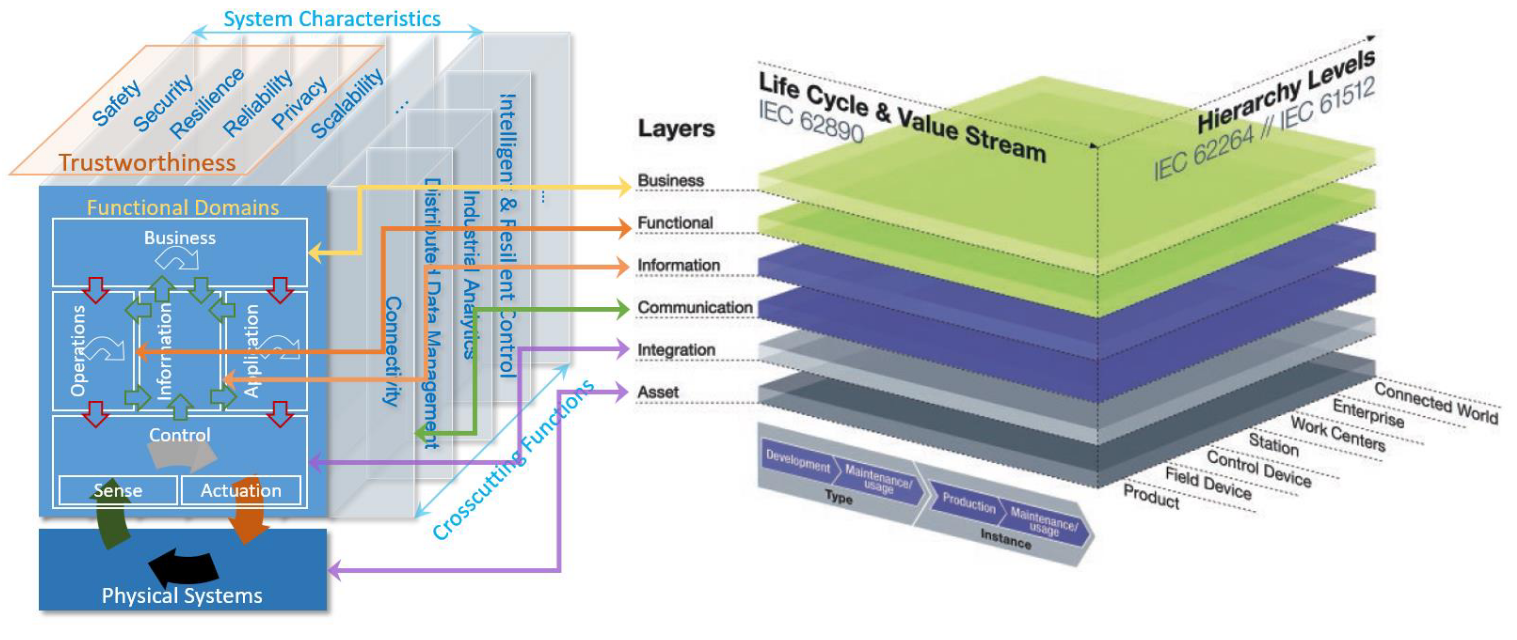
\includegraphics[scale=0.35]{
        assets/figures/iira-rami-mapping.png
    }
    \caption[IIRA and RAMI 4.0 Functional Mapping]{IRRA and RAMI 4.0 Functional Mapping, \cite{iira-inter-rami}}
    \label{fig:stateofart:arch:rami:mapping}
\end{figure}

The need to map the concepts of both reference architectures derives from the fact that these two are the most actively references used in the industry \parencite{DIAS2022100529}. Therefore, the document by \cite{iira-inter-rami} provides guidelines on how to achieve better interoperability between systems built according to different reference architecture. 

\subsubsection{Azure IRA}
\label{subsubsec:stateofart:arch:azure}

The \citetitleyear{azure-ira} proposes the architecture envisioned in Figure~\ref{fig:stateofart:arch:azure:ira}, this architecture relies heavily on the Azure platform services. According to \cite{azure-ira}, the recommended architecture is ``cloud native, microservice, and serverless-based''. This project's final version is dated back to April 2021.

\begin{figure}[H]
    \centering
    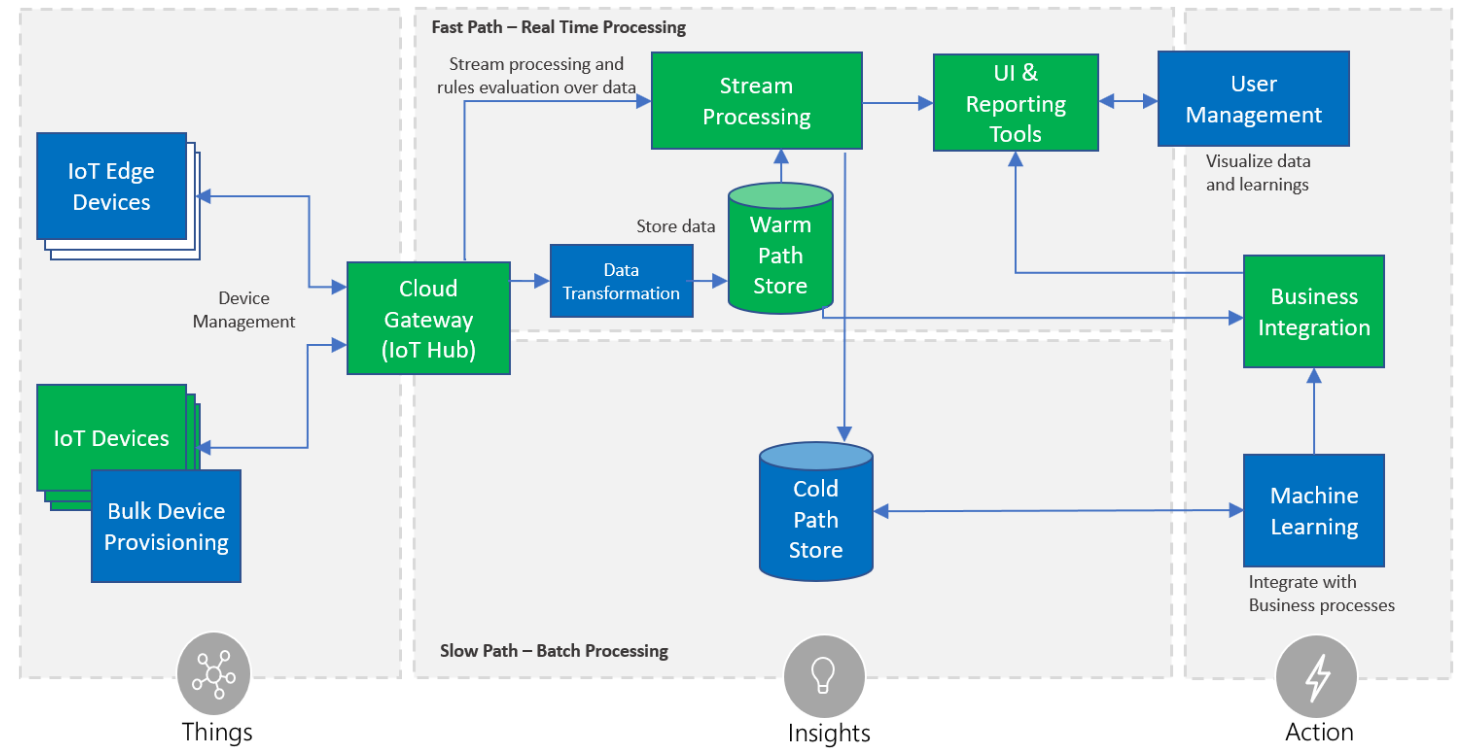
\includegraphics[scale=0.35]{
        assets/figures/azure.png
    }
    \caption[Azure IoT Reference Architecture]{Azure IoT Reference Architecture, \cite{azure-ira}}
    \label{fig:stateofart:arch:azure:ira}
\end{figure}

\cite{azure-ira} recommends that ``subsystems should be built as discrete services that are independently deployable, and able to scale independently'', to ``enable greater scale, more flexibility in updating individual subsystems, and provide the flexibility to choose appropriate technology on a per-subsystem basis''.

This reference architecture is based on the lambda architecture. According to \cite{kiran2015lambda}, the lambda architecture ``combines both batch and stream processing capabilities for online processing and handling of massive data volumes in a uniform manner, reducing costs in the process.''
It is comprised of three layers (or patches), a Batch or Slow layer for extensive and prolonged analysis, a Speed or Fast layer for real-time evident information, and a Serving layer responsible for providing the results gathered by the other two layers.

As we can see in Figure~\ref{fig:stateofart:arch:azure:ira} the Insights section is divided into two patches, the Fast Patch for real-time processing, and the Slow Patch for batch processing. Results are then provided in the Action section.

\subsubsection{Arrowhead}
\label{subsubsec:stateofart:arch:arrrowhead}

According to \cite{varga2017making}, ``the objective of the Arrowhead Framework is to efficiently support the development, deployment and operation of interconnected, cooperative systems. It is based on the \gls{SOA} philosophy''. It has a big focus on Interoperability between systems and services already in production.

``The Arrowhead project targets five business domains; Production (process and manufacturing), Smart Buildings and infrastructures, Electro mobility, Energy production and Virtual Markets of Energy'' \parencite{blomstedt2014arrowhead}.

The Arrowhead challenge is to enable interoperability between these systems, therefore, it starts by defining how one should document his/her solutions. Three hierarchical levels of solutions are proposed: (i) service, (ii) system, (iii) system of systems (Figure~\ref{fig:stateofart:arch:arrowhead:levels}).

\begin{figure}[H]
    \centering
    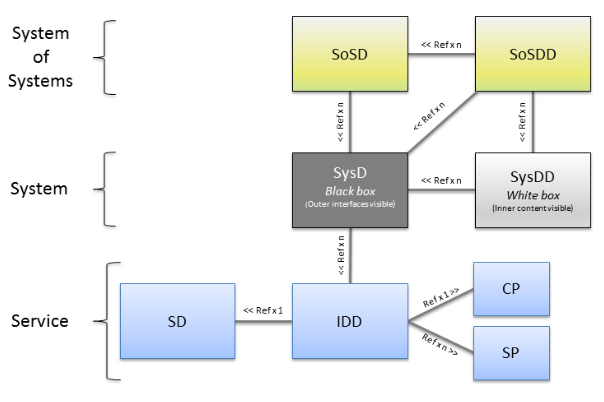
\includegraphics[scale=0.6]{
        assets/figures/arrowhead-levels.png
    }
    \caption[Arrowhead Framework Core and Application Services]{Arrowhead Framework Core and Application Services, \cite{blomstedt2014arrowhead}}
    \label{fig:stateofart:arch:arrowhead:levels}
\end{figure}

The lower level, service, can be something that, for example, indicates the current measured humidity level by sensor \textit{X} (pull-typed service) or that opens/closes valve \textit{Y} (push-typed service). A system is composed by several services. A System of Systems is composed by several systems that work in harmony in a Arrowhead local cloud. A Arrowhead local cloud is composed by at least three mandatory core systems: (i) ServiceRegistry system, (ii) Authorization system and (iii) Orchestration system presented in Figure~\ref{fig:stateofart:arch:arrowhead:system}.

\begin{figure}[H]
    \centering
    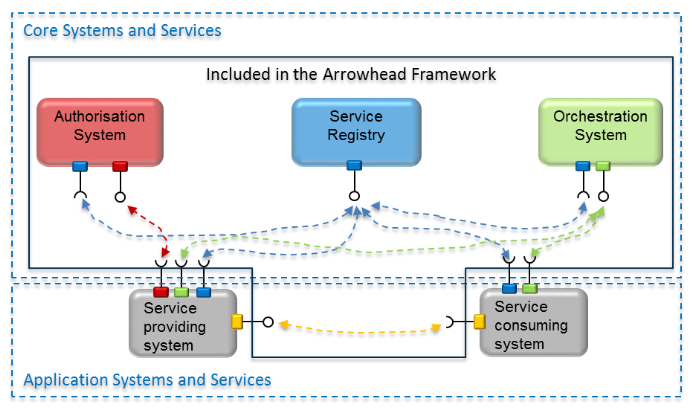
\includegraphics[scale=0.6]{
        assets/figures/arrowhead.png
    }
    \caption[Arrowhead Framework Core and Application Services]{Arrowhead Framework Core and Application Services, \cite{blomstedt2014arrowhead}}
    \label{fig:stateofart:arch:arrowhead:system}
\end{figure}

These core systems handle essential features for a local cloud such as: service discovery, service registration, service advertisement, authentication of consuming services, data exchange between systems and service coordination according to \cite{marcu2020arrowhead}. A local cloud can expose its systems to other local clouds and consume other local clouds systems. Since each service and system is well documented and arrowhead compliant it's possible to ensure interoperability between local clouds.

\subsubsection{Overall Perspective}
\label{subsec:stateofart:arch:prepective}

To close this section, some of the author sentiment and ideas surrounding these reference architecture models, and how they may shape this project's solution, are presented:

\begin{itemize}
    \item \nameref{subsubsec:stateofart:arch:iota}: The Unified Requirements detailed by this initiative gave the author an idea of the basic features for an \gls{IoT} system and enriched the requirements proposed by the company;
    \item \nameref{subsubsec:stateofart:arch:sat}: The extendability notion behind the "Embedded IoT Application" component was interesting to author from a business point of view. This idea would give customers the possibility to integrate custom-made solutions in the platform;
    \item \nameref{subsubsec:stateofart:arch:iira}: The author argues that the clear division between the Application, Information and Business domains provide a common abstraction that can be applied to any \gls{IoT} System to ease the cognitive burden taken to understand it;
    \item \nameref{subsubsec:stateofart:arch:wso2}: The author finds the clear division between the responsibilities of gathering measures, processing and analyzing them, and providing them in a business focused manner very aligned with this project's goals;
    \item \nameref{subsubsec:stateofart:arch:p2413}: The concept of "Smart City Platform", and how it interacts with various systems is highly related with the overall requirements of this project;
    \item \nameref{subsubsec:stateofart:arch:rami}: This reference architecture provided no relevant insight for the author, mostly due to the discrepancy between the \gls{IoT} domains each project was devoted to (Smart Cities vs Industry 4.0);
    \item \nameref{subsubsec:stateofart:arch:azure}: This reference architecture presented the author with a conceivable architecture for the future of the current solution. It introduced the notion of a Batch layer to better handle complex and prolonged analysis and provide \gls{KPI} reports;
    \item \nameref{subsubsec:stateofart:arch:arrrowhead}: This reference architecture appeared to be out-of-scope for the project since it focus on a more fine-grained access and control of devices (without the need for a \gls{IoT} Midlleware that handle device management and propagation of measures).
\end{itemize}

\subsection{Synopsis}
\label{subsec:stateofart:synopsis}

This section introduced the reader to the technological landscape of \gls{IoT}. The next section discusses some of its business areas or domains.

\section{Business Areas}
\label{sec:stateofart:areas}

Even though there's no concise structure, it is obvious that the \gls{IoT} technologies can be used in a broad range of areas/sectors. According to \cite{nivzetic2019smart}, the most valuable areas are: Smart Cities, Industrial \gls{IoT}, Connected Health and Smart Homes. The general market division of IoT technologies is presented in Figure~\ref{fig:iot-areas}.

\begin{figure}[H]
    \centering
    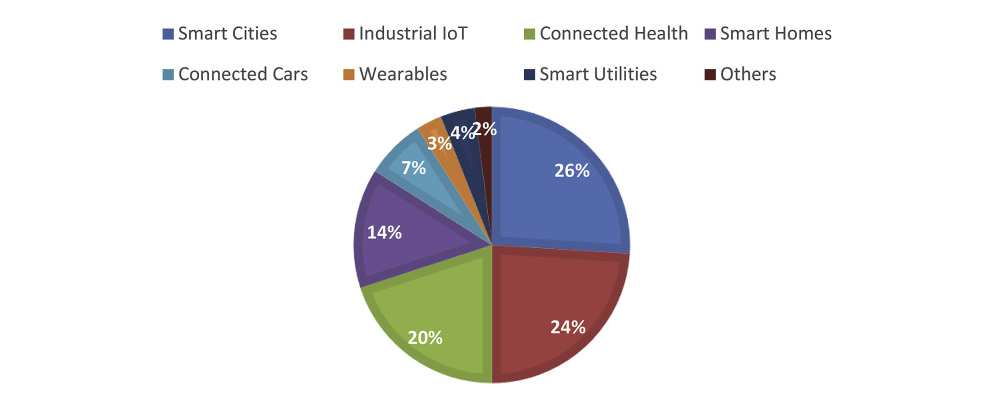
\includegraphics[scale=0.5]{
        assets/figures/iot-areas.png
    }
    \caption[IoT market structure]{General market structure of IoT technologies, \cite{nivzetic2019smart}}
    \label{fig:iot-areas}
\end{figure}

From another point of view, and according to \cite{7073822}, the sectors \gls{IoT} is related to are: Energy, Smart City, Transportation, Smart Home, Environment, Supply Chain, and Health Care.

According to (\cite{6851114}) these are the main application fields for \gls{IoT} in China: industry, smart agriculture, smart logistics, intelligent transportation, smart grids, smart environmental protection, smart safety, smart medical and smart home.

Even though this work focus mostly on Smart Cities other areas are also be described. Each of this areas incorporate several interconnected use cases that are briefly described in the following segments.

\subsection{Smart Cities}
\label{subsec:stateofart:areas:cities}

The Smart Cities sector includes numerous use cases related to public safety, the environment, mobility, energy, infrastructure and many other municipal concerns. According to \cite{iot-smart-city-prioritized} this are the use cases being prioritized.

\begin{itemize}
    \item Connected Public Transport: real-time monitoring of public transportation vehicles' locations, stops and itineraries, and the possibility to be notified when a public transportation vehicle is arriving at a stop;
    \item Traffic Monitoring and Management: real-time monitoring and management of traffic flows in a efficient manner;
    \item Water level / Flood Monitoring: real-time monitoring of level of water in public water basins such as rivers, channels, or even lakes and seas to warn and predict fast water level shifts;
    \item Video Surveillance \& Analytics: real-time monitoring using \gls{CCT} cameras and analytics to detect specific situations, e.g. accidents, crimes, potential threats, or recognize specific features (face recognition, demographics, etc.);
    \item Connected Streetlights: real-time monitoring and management of streetlights' health status and energy consumption to decrease costs and become more sustainable;
    \item Weather Monitoring: real-time monitoring of weather conditions such as temperature, humidity, rainfall, wind speed and direction to predict the weather and future natural disasters;
    \item Air Quality / Pollution Monitoring: real-time monitoring of air quality to warn the community about hazardous conditions;
    \item Smart Metering - Water: remote real-time monitoring of water usage in homes to address the world's water demand and scarcity issues and faster localize sewage leaks;
    \item Fire / Smoke Detention: real-time monitoring of possible indoor fires and CO2 levels to prevent injuries, fatalities and building degradation;
    \item Water Quality Monitoring: real-time monitoring of water conditions such as pH levels, percentage of salts and other elements that can threaten the public health.
\end{itemize}

Apart from these use cases, others are arising, such as smart parking (\cite{GOAP201841}), smart irrigation (\cite{7562735}) and waste management (\cite{7972276}).
\begin{itemize}
    \item Smart parking provides a simple method to the community of knowing the available parking spots, which, alone, lowers the carbon footprint and traffic congestions in cities.

    \item Smart irrigation tackles the need to save water by irrigating the soil only when needed and not when it is already moist, it's raining or it is expected to rain in the following hours.

    \item Waste management can eliminate the cost of unnecessary waste collections and therefore reduce the carbon footprint. Data gathered can then help to identifying cost-effective itineraries to collect waste and eventually lower overall transportation and staff costs.
\end{itemize}

All this use cases refine the efficiency of the municipal workforce and help the town council to reduce costs and improve the environment sustainability in the long term.

\subsection{Industry}
\label{subsec:stateofart:areas:industry}

According to \cite{iiot}, ``the Industrial \gls{IoT} provides a way to get better visibility and insight into the company's operations and assets", therefore this leads to ``operational efficiency gains and accelerated productivity, which results in reduced unplanned downtime and optimized efficiency, and thereby profits"".
It is comprised of several use cases (\cite{iiot-cases}) such as:

\begin{itemize}
    \item Predictive Maintenance: real-time monitoring of equipment conditions and applied data analytics can help a company to significantly decrease operational expenditures. ``Other potential advantages include increased equipment lifetime, increased plant safety and fewer accidents with negative environmental impact"" (\cite{iiot-cases});
    \item Smart metering: real-time monitoring of energy, water or natural gas consumption of a building can reduce operating expenses by managing manual operations remotely, reduce energy theft and improve forecasting and streamline power-consumption (\cite{metering-sierra});
    \item Asset tracking: real-time monitoring of resources helps "to easily locate and monitor key assets, along the supply chain (e.g. raw materials, final products and containers) to optimize logistics, maintain inventory levels, prevent quality issues and detect theft" (\cite{iiot-cases}).
    \item Connected vehicles: computer-enhanced vehicles that automate many normal driving tasks can lower crash rates, and help decreasing the number of vehicles a company needs to function.
    \item Fleet management: real-time monitoring of vehicles location and conditions can help ``improving efficiency and productivity while reducing overall transportation and staff costs"" (\cite{iiot-cases}).
\end{itemize}

As we can see from the list above, the Industrial \gls{IoT} sector is focused on business efficiency and staff safety, which, as a side effect, brings environmental benefits.

\subsection{Healthcare}
\label{subsec:stateofart:areas:healthcare}

According to \cite{FIROUZI2018583} new opportunities are now arising as a result of fast-paced expansion in the areas of the \gls{IoT} and Big Data for healthcare industries. People across the globe have begun to adopt wearable biosensors, whose data is feed into the new emerging individualized health applications.
This sector incorporates numerous use cases (\cite{iot-healthcare}) such as:

\begin{itemize}
    \item Remote Healthcare Monitoring: real-time monitoring of a patient conditions such as pulse rate and heartbeat can prevent unwanted deaths;
    \item Drug management: medicine monitoring and reminder system can help the elderly to take medicine on time;
    \item Employee health management: real-time monitoring of employee's state can predict burnouts and increase a workforce productivity;
\end{itemize}

The benefits these use cases provide are a more convenient lifestyle, improvement of one life's quality, reduction in costs and increased survival rates of patients (\cite{iot-healthcare}).

\subsection{Smart Homes}
\label{subsec:stateofart:areas:home}

Visions of smart homes have long caught the attention of researchers and considerable effort has been put toward enabling home automation. However, these technologies have not been widely adopted despite being available for over three decades (\cite{iot-smarthomes}).
Based on \cite{smarthome-review} most home automation services offer the following use cases:

\begin{itemize}
    \item Smart Lighting: remote and automated control of lights inside a house can help to decrease energy wasted;
    \item Smart Air Conditioning: remote and automated control of air conditioners can keep the house comfortable while minimizing the energy wasted;
    \item Remote health monitoring: when dealing with the elderly, complex smart systems can anticipate their needs without direct human intervention;
    \item Device Automation: smart systems can turn the lights off when no one is home, open the door when an identified person arrives and must more, improving the overall comfort of the residents.
\end{itemize}

A smart home delivers various benefits such as reducing energy waste, comfort, allowing remote control of the house, monitoring of elderly patients and easy communication with health institutions (\cite{smarthome-review}).

\subsection{Open Challenges}
\label{subsec:stateofart:arch:challenges}

Even though it seems \gls{IoT} is the obvious next step for the industry, healthcare, everyone's home, public spaces/services and everything else there are some obstacles to overcome.

One of the big challenges ahead of everyone is related with antiquated ideas, tools and processes still in use today.
Each of the use cases above mentioned require a big shift in how a company works since it demands a modernization of the organization infrastructure.
\cite{tapscott2006wikinomics}, explained that ``In an age where mass collaboration can reshape an industry overnight, the old hierarchical ways of organizing work and innovation do not afford the level of agility, creativity, and connectivity that companies require to remain competitive in today's environment"".

According to \cite{7073822} this are the most important challenges regarding \gls{IoT} applications:

\begin{itemize}
    \item Technological Interoperability: achieving a seamless interaction between devices and people with devices (according to \cite{al2016iot} there's a lack of standardization in \gls{IoT} devices and technologies);
    \item Semantic Interoperability: guaranty that the devices interpret the shared information
correctly and act accordingly (improvements have to be made regarding distributed ontologies, semantic web, or semantic device discovery);
    \item Security and Privacy: improving data integrity, unique device identification, encryption and implement proper data/device ownership for legal/liability issues;
    \item Smart Things: ultra low power circuits and devices capable of tolerating harsh environments have to be developed;
    \item Resilience and Reliability: in industrial environments or in emergency use cases temporary outages cannot be accepted.
\end{itemize}

According to the author this challenges substantially lingered the growth of \gls{IoT}, an area that was expected to have a much bigger impact in day-to-day life of everyone. According to \cite{iot-cisco-prediction} there would be 50 billion of devices connected to the Internet by 2020 but \cite{statista-number-devices} reported only 8.74 billion of connected devices.

\cite{noura2019interoperability} introduced more issues in \gls{IoT} related to interoperability from different perspectives:

\begin{itemize}
    \item Device interoperability: concerned with the exchange of information between heterogeneous devices and the ability to integrate new devices into any \gls{IoT} platform;
    \item Network interoperability: concerned with information addressing, routing, security, resource optimization, \gls{QoS} and mobility support;
    \item Syntactical interoperability: concerned with the format and structure of the information exchanged between heterogeneous systems;
    \item Semantic interoperability: concerned with the meaning behind the information exchanged, heterogeneous devices can, for example, work with diverse unit measurements;
    \item Platform interoperability: concerned with heterogeneous platforms that use diverse programming languages, \gls{OS} and software architectures (also mentioned by \cite{KOO20224191, SILVA2018697, DIAS2022100529, RAY201635}).
\end{itemize}

For \gls{IoT} Technologies to deliver on the promises made by companies like Cisco or Gartner, these barriers must be surpassed.

\section{Synopsis}
\label{sec:stateofart:synopsis}

This chapter presented the big theme surrounding this work: \gls{IoT}.
Major business areas and relevant solutions/technologies for this work were introduced.

In the following chapter, \nameref{chap:requirements}, some of the business cases and challenges discussed here will be tackled.
